\section{Modelo de Banco de Dados} % ### 5.4. Modelo de Banco de Dados

Considerando as informações necessárias para o presente trabalho, e também o preparo de campo para potenciais aplicações futuras, foi elaborado um diagrama conceitual de banco de dados, que pode ser visto na Figura \ref{fig:DiagramConceitual}.

\begin{figure}[htbp]\centering
  \caption{\label{fig:DiagramConceitual} Diagrama Conceitual do banco de dados}
  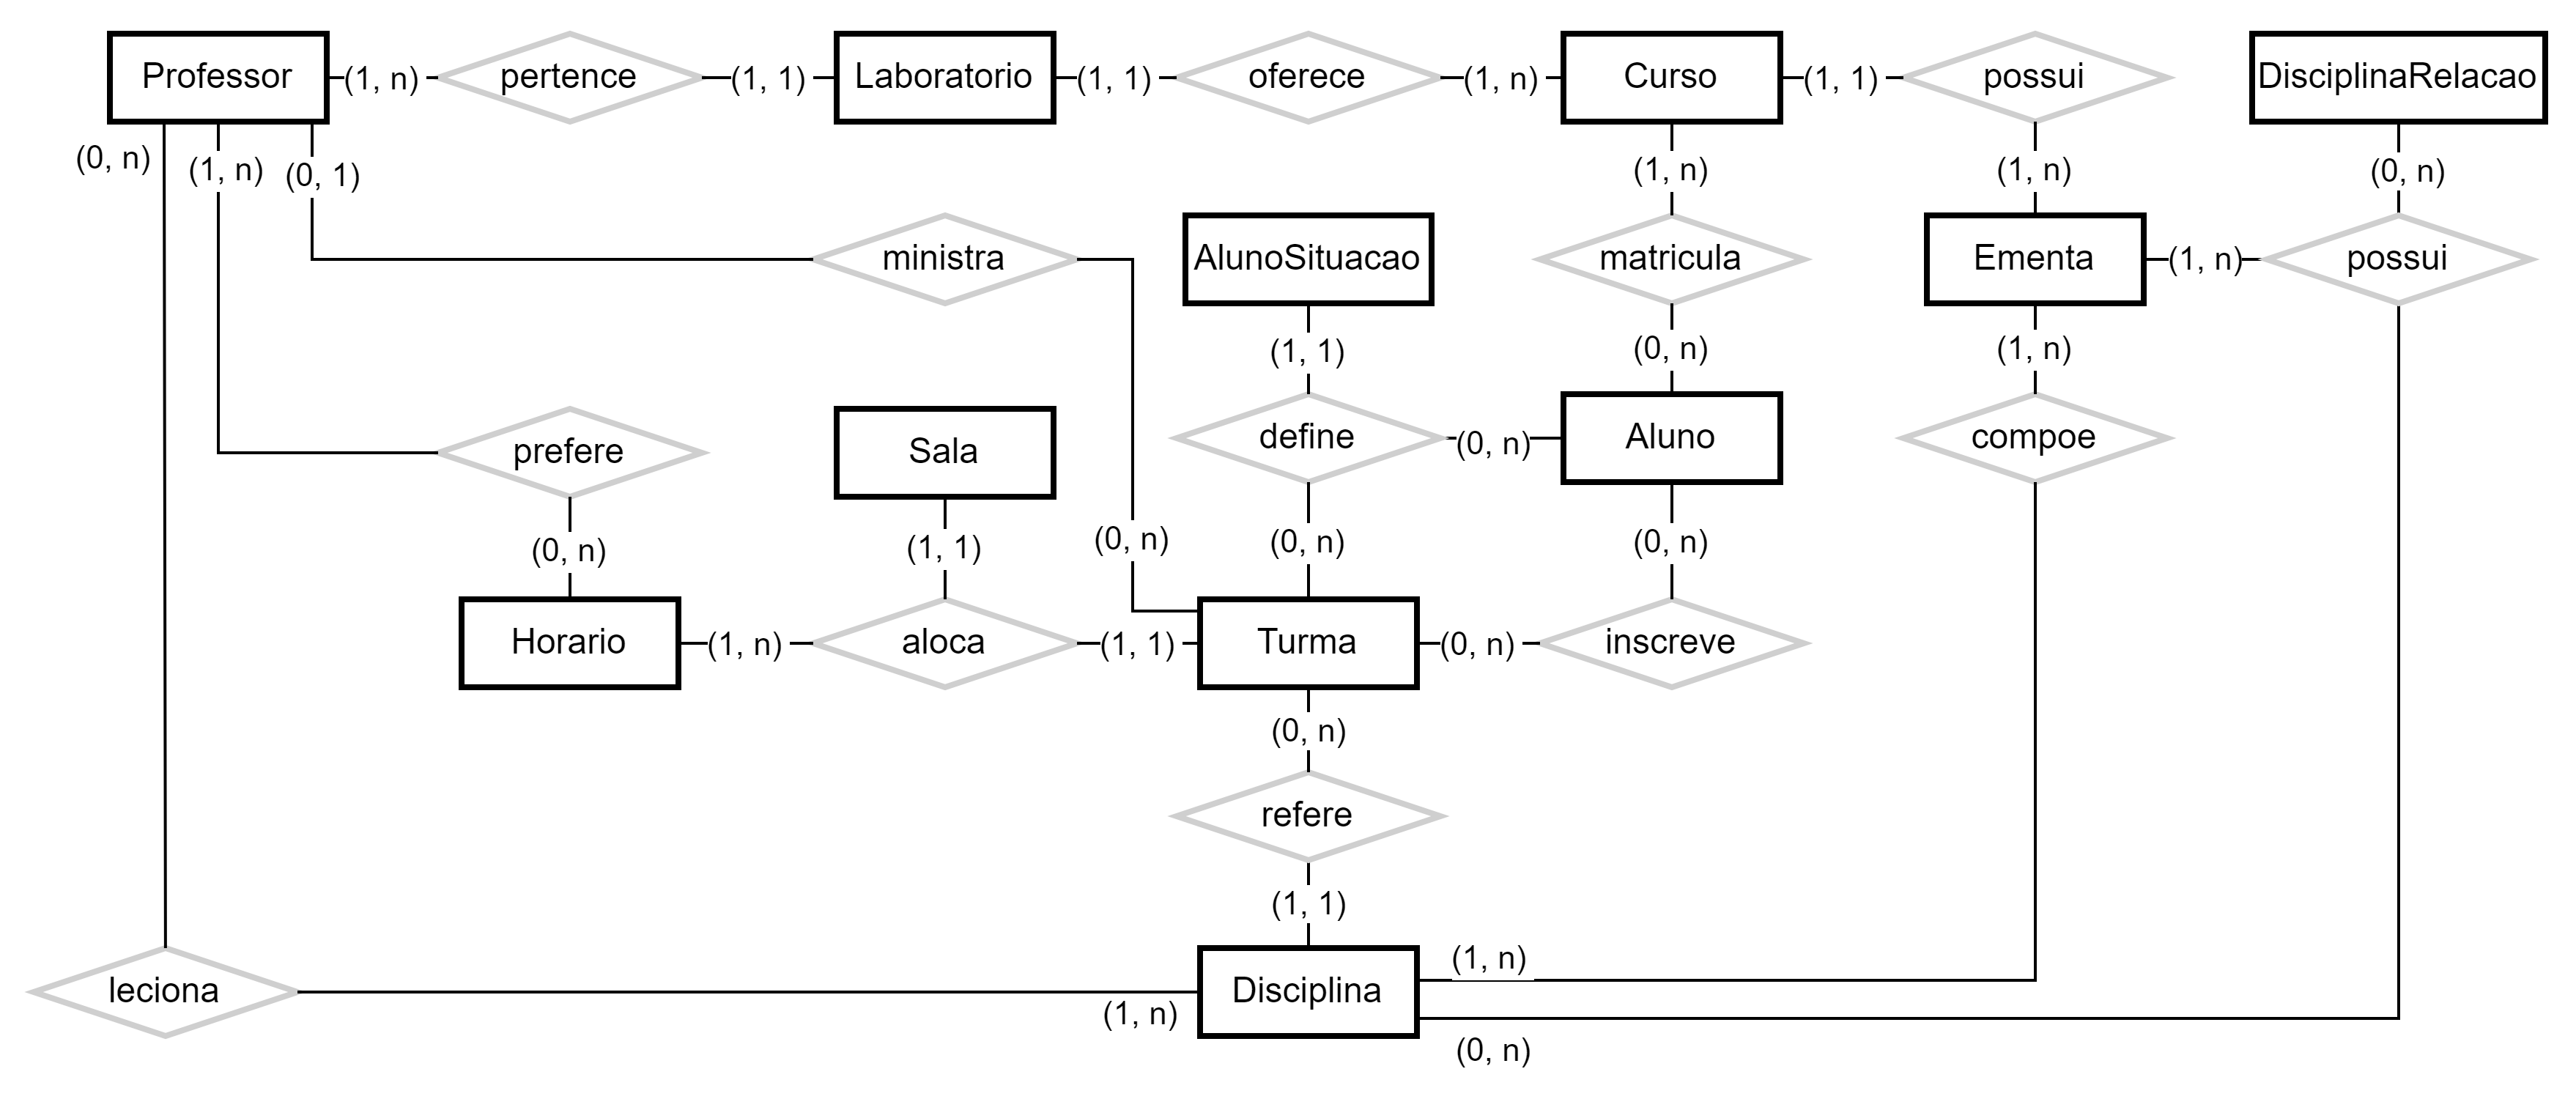
\includegraphics[scale=0.2]{files/img/DiagramaConceitual/DiagramaConceitualBranco.png}
  \legend{Fonte: o autor}
\end{figure} % Diagrama Conceitual

O diagrama conceitual foi elaborado utilizando a ferramenta \href{https://www.drawio.com/}{draw.io} citada na metodologia e ilustra as relações entre diversas entidades presentes na realidade da UENF. O emaranhamento presente no diagrama ilustra a complexidade envolvida na criação de uma grade horária, onde diversas entidades se relacionam entre si.

Como principais apontamentos, podemos citar a parte principal do modelo que é a alocação de turmas. Ela, como já descrito, envolve a correlação entre alunos de diferentes cursos, professores, disciplinas, salas e horários. Além disso, também é possível notar a presença de entidades que não são diretamente relacionadas à alocação de turmas, mas que podem se mostrar úteis, como a relação entre professores e laboratórios, e a de disciplinas e ementas.

Embora o diagrama apresente uma visão mais completa de todas as interconexões possíveis, é importante ressaltar que o presente trabalho foca primordialmente na alocação das turmas para o curso de Ciência da Computação, e que a implementação do banco de dados será feita de forma a atender a essas necessidades, fazendo então uso de uma parte do diagrama conceitual.

% Tendo isso em vista, o modelo conceitual reduzido para o presente trabalho pode ser visto na Figura \ref{fig:DiagramConceitualReduzido}.

% \begin{figure}[htbp]\centering
%   \caption{\label{fig:DiagramConceitualReduzido} Diagrama Conceitual reduzido para o presente trabalho}
%   \includegraphics[scale=0.2]{files/img/DiagramaConceitual/DiagramaConceitualReduzidoBranco.png}
%   \legend{Fonte: o autor}
% \end{figure} % Diagrama Conceitual reduzido

Neste modelo, mais enxuto, temos apenas as entidades principais, onde temos uma turma de determinada disciplina, ministrada por um professor e que ocorre em uma sala em um determinado horário.

\subsection{Diagrama de Entidade e relacionamento} % ### 5.4.1. Modelo Relacional

% Com isso, restamos o diagrama de Entidade e Relacionamento (DER) que pode ser visto na Figura \ref{fig:DER}.

% \begin{figure}[htbp]\centering
%   \caption{\label{fig:DER} Diagrama de Entidade e Relacionamento}
%   \includegraphics[scale=0.2]{files/img/DER/DERBranco.png}
%   \legend{Fonte: o autor}
% \end{figure} % Diagrama de Entidade e Relacionamento

Neste diagrama vemos as entidades principais, que são \textit{Turmas}, \textit{Disciplinas}, \textit{Professores}, \textit{Horários} e \textit{Salas}. As propriedades escolhidas para cada entidade são compostas por uma mistura de critérios. Por exemplo, o nome do professor, o código da disciplina, e a junção de código e bloco auxiliam primordialmente na identificação real dos professores, disciplinas e salas. Já as informações ``período'', ``apelido'' e ``comment''...

E também é notável a presença da entidade \textit{Alunos}, que se apresenta desacoplado das demais entidades. O motivo para isso é que, embora os alunos façam parte do processo de alocação de turmas, ao longo do desenvolvimento, o desenvolvimento de funcionalidades envolvendo os alunos...

\section{História do desenvolvimento} % ### 5.5.1. História do desenvolvimento

%% Acho que vai ficar mais fácil assim

Após a elaboração dos protótipos com o Figma, e da conceitualização diagramática do banco de dados, o desenvolvimento do sistema foi iniciado. Por maior familiaridade com a linguagem e considerando que é uma das mais utilizadas no mercado para desenvolvimento web [buscar referência], foi escolhida a linguagem JavaScript, utilizando a biblioteca React para a criação dos componentes visuais, ou seja, o front-end, e o Node.js para a criação do back-end e a criação de um servidor local que permitiria visualizar as mudanças no código em tempo real.

% Perguntar pra quem sabe, sobre qual é o real papel do Node.js

\subsection{Primeira versão} % ### 5.5.2. Primeira versão

A primeira versão do sistema foi desenvolvida em um ambiente local, com o objetivo de se aproximar ao máximo das páginas previstas no protótipo. Para isso, foi utilizada a biblioteca React Router para a navegação entre as páginas, e a biblioteca React Select para as caixas de seleção.

Os dados contidos no sistema foram inicialmente armazenados em arquivos JSON, que eram importados diretamente para o código. Isso foi feito para que fosse possível visualizar o funcionamento do sistema sem a necessidade de um banco de dados real. A partir disso, foi possível visualizar o funcionamento do sistema e realizar testes de usabilidade. Em contrapartida, os dados disponíveis não eram modificáveis, tendo apenas a possibilidade de leitura e mutação temporária, visto que após recarregar ou mudar de página, as mudanças eram perdidas.

Nessa primeira versão, algumas funcionalidades já começaram a ser esboçadas, principalmente as funcionalidades CRUD (Create, Read, Update, Delete) para as entidades principais do sistema. Embora, como já dito, os dados não fossem persistentes, foi possível visualizar o funcionamento das funcionalidades de criação e leitura de turmas, professores, disciplinas, salas e horários.

Além dessas funcionalidades que se mantiveram até a conclusão do sistema, também foram desenvolvidas funcionalidades que não obtiveram o mesmo êxito e que foram deixadas de lado ao decorrer do caminhar. Dentre elas, podemos citar a definição de níveis de preferência de horários para professores, a definição das características especiais das salas, e o andamento dos alunos em relação às disciplinas. Houveram também outras que nem chegaram a ser desenvolvidas, como a realocação de turmas através de um sistema de arrastar e soltar e o uso de heurísticas para a realocação de turmas.

Após o desenvolvimento local, como forma de viabilizar o acesso ao sistema por parte de outros usuários, foi feito o \textit{deploy}, ou seja, foi feito o upload do sistema para um servidor online. Para isso, foi utilizado o serviço GitHub Pages que, por ser gratuito e de fácil utilização, foi a escolha mais adequada para o momento. O sistema pode ser acessado através do link \url{https://jvfd3.github.io/timetabling-UENF/}.

Nessa versão, também foi implementada uma checagem bruta de conflitos por alocação simultânea de professores em mais de uma turma e a checagem da quantidade de demanda de alunos em relação à capacidade das salas.

\subsection{Segunda versão} % ### 5.5.3. Segunda versão

Utilizando do feedback quanto aos resultados entregues na primeira versão, alguns pontos de melhoria foram identificados, sendo um deles, e o mais importante: o planejamento. Na primeira abordagem, o desenvolvimento foi feito seguindo notas e ideias soltas, sem um planejamento prévio, o que resultou em um sistema que, embora funcional, não atendia a todas as necessidades propostas. E ia além: exibia funcionalidades que não eram de todo necessárias, ou melhor dizendo, têm menor prioridade do que muitas outras.

\subsubsection{GitHub Projects}

Com isso, utilizando o GitHub Projects, foi organizado uma tabela de tarefas, onde foram unificadas as diversas anotações e ideias, antes soltas. A partir disso, foi possível visualizar o que era mais importante e o que poderia ser deixado de lado.

% [ADICIONAR IMAGEM DA TABELA BONITINHA: https://github.com/users/jvfd3/projects/3]

Tendo este novo sistema de tarefas em prática, foi possível tranquilizar a mente quanto ao conflito entre as funcionalidades que precisavam ser desenvolvidas, as que já estavam prontas, as que poderiam ter melhorias e quais se desejava implementar no futuro.

As tarefas foram inicialmente divididas em três principais categorias: \textit{Status}, \textit{Pages} e \textit{Sequence}. O \textit{Status} reflete o andamento da tarefa, se ela está disponível, em andamento, ou concluída. O \textit{Pages} reflete em qual página do sistema a tarefa se encontra, e o \textit{Sequence} reflete a ordem de prioridade da tarefa.

\subsubsection{Permanência dos dados}

Tendo agora uma rota mais clara a ser seguida, o desenvolvimento foi retomado. Uma das características mais marcantes e ainda não atribuídas ao sistema era a manutenção dos dados. Como até então os dados estavam armazenados em formato JSON, imaginou-se que a melhor forma de persistir os dados seria através de um banco de dados que lidasse com JSON, e o escolhido foi o JSONBin.

Mesmo cumprindo com o que promete, o JSONBin não se mostrou a melhor escolha para o sistema, visto que a sua utilização não performou tão bem quanto se esperava. Não se sabe se foi por inexperiência ou por limitações do próprio serviço, mas a utilização do JSONBin para a coleta dos dados, fazia com que a tela de carregamento do sistema demorasse alguns segundos para ser exibida, o que não é aceitável para o sistema proposto.

\subsubsection{...}

Assim como na primeira versão, algumas funcionalidades foram desenvolvidas e outras foram deixadas de lado. Uma das que foram deixadas de lado são:
